% --------------------------------------------------------------------------
% Template by Leonard Mandla Mbuli (mail@mandla.me) & Adam Pantanowitz (adam.pantanowitz@wits.ac.za)
% School of Electrical and Information Engineering
% University of the Witwatersrand
%
% compiled with (this is assuming you are using minted):
% pdflatex -shell-escape main

% REQUIREMENTS:
% fullpage - for fullpages
% graphicx - pictures
% xcolor   - pretty colours easier naming
% minted   - for code highlighting
% url      - for urls in the the text and in references
%
% More information on minted can be found in the doc/minted.pdf
%
% created: 20 December 2011
% updated: 10 May 2014
% ---------------------------------------------------------------------------
\documentclass[11pt]{article}
\usepackage[margin=2.3cm]{geometry}
\usepackage[usenames,dvipsnames]{xcolor, colortbl}
\usepackage{graphicx}
\usepackage{url}
\usepackage{titlesec}
\usepackage{booktabs}
\usepackage{ragged2e}
\usepackage{lipsum}
\usepackage{listings}
\lstset{
  basicstyle=\fontfamily{lmvtt}\selectfont\footnotesize\color{black},
  columns=fullflexible,
}
\usepackage{multicol}
\setlength{\columnsep}{1cm}

\definecolor{myblue}{rgb}{0.0, 0.0, 0.5} % for the section headings and title
\definecolor{mylightgrey}{gray}{0.9} % for the tables

\titleformat{\section}
{\color{myblue}\normalfont\Large\bfseries}
{\color{myblue}\thesection}{0.5em}{}
%\renewcommand{\familydefault}{\sfdefault}

\begin{document}
\pagestyle{empty}
\begin{minipage}{0.18\textwidth}
    
\includegraphics[width=\textwidth,height=\textwidth]{images/eie.png}
\end{minipage}
\begin{minipage}{0.8\textwidth}
    \centering
    \textbf{\Large School of Electrical and Information Engineering}\\
    {\large University of the Witwatersrand, Johannesburg}\\
    {\small Private Bag 3, 2050, Johannesburg, South Africa}\\
\end{minipage}
\vspace{.3cm}\\
\colorbox{myblue}{\begin{minipage}{0.98\textwidth}
        \begin{center}
            \textcolor{white}{\textbf{\Large{ELEN4017: Project - 2017}}\\
                \textbf{Networks:  Email Application System}\\
                May 2017
            }
        \end{center}
    \end{minipage}
}
\\
\vspace{6cm}
\begin{center}
{\Huge Benjamin Thomas (Ben)} \\
{\Large 545787} \\
{\large 545787@students.wits.ac.za}
\break{}
\break{}
{\Huge Benjamin Shear (Benji)} \\
{\Large 749992} \\
{\large 749992@students.wits.ac.za}
\end{center}
\vspace{1cm}
\begin{abstract}
\justify In this project the features of an email application were implemented. An email system comprised of an IMAP (Internet Message Access Protocol) client and server, POP3 (Post Office Protocol 3) client and server, and SMTP (Simple Mail Transfer Protocol) client and server was developed. The system also contains a Graphical User Interface (GUI) for some of the functionality as well as demonstration scripts to automate the system. The report will discuss the structure, features, response and replies, code and critical analysis of the system.
\end{abstract}
\newpage
\begin{multicols}{2}
\section{Introduction}
Email plays a vital role in the day to day functioning of modern society. As one of the building blocks of the early internet, email has remained surprisingly relevant today as ever - despite the introduction of messaging technologies such as SMS, Whatsapp, Telegram and iMessage. Therefore, this project involves the investigation, design and implementation of an emailing system based on the robust protocols that define Email communication.
\section{Implemented System and Overview of Features}
The system implemented consists of an email client and email server.  The system design was guided by the Request for Comments (RFC) publications as per the Internet Engineering Task Force and the Internet Society. The client side allows for communicating with an email IMAP server by the TCP protocol at the transport layer and using the IMAP protocol at the application level. The IMAP protocol was partially according to RFC 3501. The system also allows for interacting with an SMTP server to send email via the SMTP protocol. The SMTP server is a multithreaded server allowing for it to communicate with multiple client TCP connections simultaneously. The SMTP sever has the ability to relay any emails sent to it to another SMTP server. The SMTP design  was partially according to RFC 5321. A multithreaded IMAP server was implemented which has the ability to interpret commands sent to it and respond according to the IMAP protocol. With POP3, a similair structure as IMAP with regards to the client and server was deployed. However, at the time of submission the code has not been fully tested and is therefore meant to mainly give an idea to the structure of the POP3 system as opposed to an actual implementation. The POP3 design was partially according to RFC 1393.
\\\\
The system  makes use of a simple GUI to demonstrate some of the functionality and help the user easily navigate through the application. To further demonstrate the workings of the servers and clients a number of demonstration scripts have been created. These scripts, with minimum modification can run client/servers to demonstrate certain key functionality.
\subsection{Missed features}
The application is able to effectively send and receive emails, however the application is not able to handle email attachments and only is able to handle text in the body of the email. Additionally many of the commands and specifications for formatting as specified in the RFC were not implemented. In most cases the bare functionality needed to perform basic email client and server tasks were implemented. In the case of the IMAP and POP3 servers the server only replies to a limited number of requests and does not have the ability for real email to be transferred onto these servers. Rather, mock accounts and emails have been set up in the code for demonstrative purposes.
\section{Protocols}
Below are the client commands and server response codes that have been implemented in the code.
\subsection{SMTP}
\subsubsection{SMTP Client Commands}
\begin{itemize}
  \item \textbf{EHLO localhost} - Sends the EHLO command as per SMTP protocol.
  \item \textbf{AUTH LOGIN} - Sends the request to login. The server then responds, requesting client to send username and password.
  \item \textbf{MAIL FROM: [argument]} - Requests the senders mail ID.
  \item \textbf{RCPT TO: [argument]} - Requests the receivers mail ID.
  \item \textbf{DATA} - Requests the data to be sent. The server interprets a full-stop on an empty line as the token that informs the server when the client has finished sending data.
  \item \textbf{NOOP} - Requests for the server to reply with a '250 OK'.
  \item \textbf{VRFY [argument]} - Verifies if a user exists on the server.
  \item \textbf{RSET} - Abort current mail transaction.
  \item \textbf{QUIT} - Terminate session with server.
\end{itemize}
\subsubsection{SMTP Server Replies}
\begin{itemize}
  \item \textbf{250 Hello, I am delighted to meet you} - Sent upon receiving EHLO from client 
  \item \textbf{250 Ok} - sent in reply to the following cases: MAIL FROM: [argument],RCPT TO: [argument], after an email has been relayed.
  \item \textbf{354 End data with $<$CR
  \\$>$$<$LF$>$.$<$CR$>$$<$LF$>$} - Sent in response to DATA command. 	
  \item \textbf{221 Bye} - Sent in response to QUIT command from client \cite{SMTP}. 
\end{itemize}
\subsection{POP3}
\subsubsection{POP3 Client Commands}
\begin{itemize}
  \item \textbf{USER [argument]} - This allows the user to pass their user-name to the POP3 server for authentication
  \item \textbf{PASS [argument]} - This allows the user to pass their password to the POP3 server for authentication against the user-name already entered
  \item \textbf{STAT} - This allows the user to view how many emails are in the inbox as well as the size (number of bytes) of the inbox
  \item \textbf{LIST [argument]} - This allows the user to view the size of a specific email. If no argument is passed, the server returns the size of each email in the inbox.
  \item \textbf{RETR [argument]} - This allows the user to retrieve a specific email corresponding to the argument passed in.
  \item \textbf{NOOP} - This does nothing.
  \item \textbf{DELE [argument]} - This marks a user specified email for deletion.
  \item \textbf{RSET} - This clears all emails that have been marked for deletion.
  \item \textbf{QUIT} - This closes the connection.
\end{itemize}
\subsubsection{POP3 Server Replies}
\begin{itemize}
  \item \textbf{+OK Send PASS} - In reply to USER [argument]
  \item \textbf{+OK Welcome} - In response to PASS [argument] if the password matches the user-name, and \textbf{-ERR [AUTH] Username and password not accepted} if it does not.
  \item \textbf{+OK [number of messages in inbox] [size (in bytes) of inbox]} - in response to STAT.
  \item  \textbf{+OK [message number] [size (in bytes) of message]} - in response to LIST [argument]. or \textbf{-ERR Message number out of range} if the argument passed is larger than the number of messages on the server.
  \item The server will either reply with the content of the message or \textbf{-ERR Message number out of range} if the argument passed is larger than the number of messages on the server in response to RETR [argument].
  \item \textbf{+OK} - In response to NOOP.
  \item - \textbf{+OK Message marked for deletion} - in response to DELE [argument]  or \textbf{-ERR Message number out of range} if the argument passed is larger than the number of messages on the server.
  \item \textbf{+OK} - in response to RSET.
  \item  \textbf{+OK Farewell} - in response to QUIT \cite{POP3}.
\end{itemize}

\subsection{IMAP}
\subsubsection{IMAP Client Commands}
\begin{itemize}
  \item \textbf{LOGIN [username] [password]} - login to IMAP server using username, password.
  \item \textbf{SELECT INBOX} - Display details of messages.
  \item \textbf{CAPABILITY} - Request from server to send back its functionalities.
  \item \textbf{LIST INBOX} - List folders in INBOX.
  \item \textbf{DELETE inbox} - Delete folder 'inbox'. 
  \item \textbf{FETCH [argument]} - get body/header of emails requested.
  \item \textbf{SUBSCRIBE [argument]} - Subscribe to a mailing list.
  \item \textbf{UNSUBSCRIBE [argument]} - Unsubscribe to mailing list.
  \item \textbf{CLOSE} - Terminate session with server.
  \item \textbf{COPY} - Copy specified emails to a folder
  \item \textbf{LOGOUT} - Logout from logged in session. 
\end{itemize}
\subsubsection{IMAP Server Replies}
\begin{itemize}
  \item \textbf{Ok LOGIN completed} - in reply to successful LOGIN [username] [password].
  \item \textbf{* [MAILBOX] exists} - in reply to SELECT INBOX. 
  \item \textbf{Messages: [messages]} - in response to  FETCH  
  \item \textbf{No login failure: username or password rejected} - in reply to unsuccessful LOGIN [username] [password] \cite{IMAP}. 
\end{itemize}
\section{Detailed Feature Implementation}
\subsection{Socket Handling}
The IMAP, SMTP and POP3 clients have the ability to connect to their respective destination servers on the relevant port using Secure Sockets Layer. Once the client is able to establish a TCP socket connection with the destination server the socket handling functionality takes in a string passed to it from the application level. It then passes this to the TCP stream and sends to server. The response from the server will be received from the stream and passed to the application.
\\\\
Likewise, the respective servers implemented have the ability to receive TCP connections from multiple hosts. The programme sets up a listener for incoming connections to a single port. In the case where a client connect to the server port, it establishes an SSL connection with them and; it has a public key and self signed certificate to authenticate to the client. One the connection is made the programme designates a socket and its own thread to that client and all future connections are via that designated port. 
\subsection{IMAP Client}
The IMAP client has the ability to format strings for sending based on the IMAP protocol - such as appending each sent message to the server with an alphanumeric string and ending the message with Carriage Return and new line characters. The client functionality provides the user the ability to authenticate itself to the server and to view the server's capabilities. It can select mailboxes and list folders in the inbox. It can then select and view the header and body of the emails.
\subsection{IMAP Server}
The server does not provide the ability for the user to view a real email account. Rather a mock user has been set up in the code with mock emails. An email client may interact with the IMAP server and can only authenticate with that particular 'user account'. If the client requests to see the messages, the IMAP server will return them - however they are not in the format of a typical email. Rather, for demonstration purposes a string, with details of the sender and the actual message is sent back to the client upon request.
\subsection{SMTP Client}
The SMTP client code provides the user with the ability to authenticate him or herself to the server, sending the username and password base64 encoded. It provides the ability to send an email to the SMTP server, allowing for specifying of the recipient and sender as well as the body of the message.
\subsection{SMTP Server}
The SMTP server has the ability to receive input from the client's side and interpret the client's commands. The incoming command from the client is parsed and classified as a certain SMTP command accordingly. The SMTP can interpret and respond to commands such as EHLO, MAIL FROM, RCPT TO, and QUIT. Upon receiving a RCPT TO command the server will store the address of the recipient. The server then in turn becomes a client to another SMTP server (in the demonstration case - smtp.gmail.com) and will authenticate itself to that server and send an email to the server with the MAIL FROM being that of the relay server itself and the RCPT TO being that of the original senders email. The message pasted after the original DATA request is copied and then sent onto the next SMTP server.
\subsection{POP3 Client and Server}
Similar functionality as to that of the IMAP client and server was coded. However, at the time of submission the code had not been fully tested and is therefore not run in the demonstration code.
\subsection{Graphical User Interface}
Figure 1 of Appendix A shows the screen presented to the user upon running the application. The left half of the screen represents the receiving half of the screen and the right half of the screen represents the sending half of the screen. The user is first required to enter their user-name and password into the 'Username" and 'Password' fields, before clicking the 'Login' button. A pop-up message appears and indicates if the user-name or password are correct or incorrect. If correct, the program logs into the corresponding SMTP server.
\subsubsection{Mail}
As mentioned earlier, the right half of the screen represents the sending half of the screen and will be discussed in this section. Seeing that the user has already logged into the SMTP server, the user simply needs to type in the recipients email ID and the content of the email in order to send an email. Figure 3 in Appendix A shows the user networks4017tester@gmail.com logged in, sending an email to benjaminthomassa@gmail.com with the content of the message being some dummy text. If the message is able to send successfully, a pop-up message is displayed informing the user that the message has been successfully sent as shown by Figure 3.
\subsubsection{Receiving mail}
If the user wishes to receive mail, then the user needs to either select the IMAP or the POP3 check box. Upon doing so, the program will then either log into the IMAP or POP3 server, depending on which the user selected. This is shown by Figure 4 and 5, where the IMAP and POP3 servers were logged into respectively. If the user opted to log into the IMAP server, the drop-down box will contain items that correspond to the IMAP protocols and if the user opted to log into the POP3 server, the drop-down box will contain items that correspond to the POP3 protocols. Certain protocols (such as the POP3 RETR protocol) require the user to input additional data, in which case the user needs to enter the data into the 'Command' box. Once all the required fields have been selected or filled, the user can then hit the 'Send Command' button, which will send the command that the user has chosen, to the corresponding server (IMAP or POP3). The interaction between the client and server is displayed in the Text Area at the bottom half of the receiving half of the screen. Figure 6 in Appendix A shows the Text Area being filled when a POP3 RETR protocol is run. The dummy text that was sent earlier can be seen, showing that the program is able to both send and receive emails.
\section{Division of work}
The work was divided as follows:\\
\break{}
\begin{tabular}{ |p{3cm}||p{1.5cm}|p{1.5cm}|}
 \hline
 \multicolumn{3}{|c|}{Percentage Division Of Work} \\
 \hline
  & Ben & Benji\\
 \hline
 SMTP & 0 & 100\\
 IMAP & 0 & 100\\
 POP & 100 & 0\\
 Multithreading & 0 & 100\\
 GUI & 100 & 0\\
 Report & 80 & 20\\
 \hline
\end{tabular}

\section{Results}
The Demonstration files were run and wireshark captures were taken of the programme running. All figures reffered to in this section can be found in Appendix B. All Python scripts referred to in this section are found in the Demonstration folder of the code. Fig. \ref{IMAP_CLIENT} shows a wireshark capture of the interaction between the running IMAP client (IP address 192.168.43.112) and that of imap.gmail.com (IP address 64.233.167.108). The file IMAPClientDemons.py was run to automate the client side interaction. Fig. \ref{IMAP_SERVER} show the interaction between the IMAP client (run in IMAPserverDemo\textunderscore 2.py) and the IMAP server (run in IMAPserverDemo\textunderscore 1.py). The client  programme which automates some client commands was run by the computer of IP adress 192.168.66.219 and the server programme was run on another computer (in the same network) at IP address 192.168.66.184. Fig. \ref{SMTP_CLIENT} shows the interaction between the SMTP client (run in SMTPclientDemo.py at IP address 192.168.1.14) and the server smtp.gmail.com (IP address 74.125.206.109). SMTPclientDemo.py automates client side SMTP commands. Fig. \ref{SMTP_SERVER} shows the interaction between a SMTP client run on 192.168.66.219 and the SMTP server (SMTPserverDemo.py) run on 192.168.66.184.
\section{Critical Analysis}
The structure of the project may contain certain redundancy in code as much of the code across the servers was repeated in each case. Likewise for the clients. The implementation of the system is also minimal in that it was designed to provide minimal functionality and mainly for demonstrative purposes. On the other hand, by taking a modular approach to the design and separating the GUI, socket handling and client/server code it has been easy to interface and make changes between the system components and it allows for future scale and adding of more functionality.
\section{Code structure}
The project was coded in Python 2.7 and is designed to run on a Linux operating system. The main directory consists of four folders - Client, Server, GUI and Demonstration. A file called ServerClientDetails.py found in the main directory functions as a configuration file as to the ports and destination and/or source addresses of the servers and clients. All Client and Server functionality refer to this file to configure their addresses and ports. This section will discuss the class structure within each separation, as well as some of the important methods.

\subsection{Server}
\subsubsection{ServerHandler Classes}
The ServerHandler.py file contains classes for handling server interactions at the TCP level. The SMTPsocketThreadHandler, IMAPsocketThreadHandler and POPsocketThreadHandler classes deal with opening up the server socket port for connections and binding a listener for incoming connections. Once a connection has been received  the socket thread handler will associate an SMTPserver\textunderscore thread, IMAPserver\textunderscore thread or POP3server\textunderscore thread respectively with each incoming connection. The server\textunderscore thread classes are responsible for designating each client making a connection its own port for subsequent interactions. Once the thread has started it will run an infinite loop that will continuously receive input from the TCP stream from the client and interpret and respond to this data until the client terminates the connection. Each server\textunderscore thread object created (for the designated connection) will have its own instance of an IMAPserver, SMTPserver and POP3server object. This is discussed in the following section. 
\subsubsection{SMTP/IMAP/POP3server Classes}
The SMTPserver, IMAPserver and POP3server classes contain code that interprets incoming messages passed to it by the server\textunderscore thread classes and will parse the data, and according to the command received will respond with a reply code (SMTP) or the alphanumeric identifier (IMAP and POP3) with the response text appended to this. Each server\textunderscore thread has its own instance of the server class which keeps track of the state of the current connection. Each server class has an 'interact' function which checks the received message against a number of conditions and if the condition is met the server class calculates a response and passes this response string back to the server\textunderscore thread which then inserts it into the TCP stream to be received by the client.

\subsubsection{How to set up a Server}
To set up a server, a POP3/IMAP/SMTP-socketThreadHandler object must be instantiated. Once this has been done the server is ready and will wait for incoming connections to the designated port for processing.

\subsection{Client}
The client division was subdivided into separate sections according to the functionality of each section. This consisted of a client\textunderscore sockets, a SMTPclient, a POP3client and a IMAPclient.
\subsubsection{client\_sockets class}
The client\textunderscore sockets.py file contains 3 classes which allocate TCP sockets on the client side for the SMTP, POP3 and IMAP services. These classes are clientIMAPSocket, clientSMTPSocket and clientPOP3Socket. These classes set up a socket that connects with the various remote server on the port of the service needed. For SMTP (SSL) the program connects to port 465 for the TCP connection. For IMAP, the program connects to port 993 and for POP3, the program connect to port 995. Each class has a sendMessageReceiveReply function that takes in a string as an argument, formats it correctly so that it can be sent via TCP stream to the server and it returns the reply of the server. Each SMTP/IMAP/POP3-client class contains a client\textunderscore sockets object instance. The sendMessageReceiveReply method of the client\textunderscore sockets object is then used by the client at the application level to pass data to the transport layer.
\subsubsection{SMTPclient Class}
The SMTP client class is responsible for interacting with the SMTP server. The class creates a client socket object to establish a connection with the SMTP server socket. The class has to follow all SMTP protocols, such as sending an EHLO command, before authentication can occur. The class has the primary ability to authenticate the user's user-name and password with the SMTP server as well as to send data from a sender to a receiver. The function authenticate() works by first encoding the user's user-name and password. A 'AUTH LOGIN' message is then sent to the SMTP server so that the server knows to expect the encoded user-name and password from the client.
\subsubsection{IMAPclient Class}
The IMAP client class is responsible for interacting with the IMAP server. The class creates a client socket object to establish a connection with the IMAP server socket. The class has the primary ability to authenticate the user's user-name and password with the IMAP server as well as to send data from a sender to a receiver. The function LOGIN() works by sending the user's user-name and password to the IMAP server, preceded by the word 'login'. If authenticated, the client then has the ability to carry out the LIST, DELETE, LOGOUT, SELECT and FETCH functions which are all self-explanatory.
\subsubsection{POP3client Class}
The POP3 client class is responsible for interacting with the POP server. The class creates a client socket object to establish a connection with the POP3 server socket. The class has to follow all POP3 protocols, such as first sending an USER command, with the client's user-name passed in as a parameter. The server then requests a password from the client before validating the user-name and password. The client sends the password through the PASS function, with the password being passed in as a parameter. Once authenticated, the client then once again has the ability to carry out the LIST, DELETE, RETRIEVE, RESET and QUIT functions. The only function which needs clarification is the LIST function, which has the option to either pass in an argument or not to. If an argument is passed in, then the server will list that specific email (the size of the email in bytes), if not then the server will list every single email belonging to the client with each corresponding email size (in bytes).
\subsection{Graphical User Interface}
The Graphical User Interface division was subdivided into separate sections according to the functionality of each section. This consisted of a GUI, a SMTPfunctions, a IMAPfunctions and a POP3functions file. The GUI file is responsible for presenting an easy to use graphical interface and each of the function files are responsible for linking the SMTP, IMAP and POP3 servers to the GUI. The GUI file makes use of the Tkinter package to form the graphical user interface. The GUI uses an array of Tkinter objects such as buttons, text boxes, check boxes, combo boxes and labels to form the GUI that is visible to the user.

\subsection{Demonstrations}
A number of demonstration scripts have been placed in the Demonstration file that are there to be run, and demonstrate interactions of the client/server. Each file contains specific instructions for how to run the demonstrations - such as requirement to run as super user, order to run them and in some cases the necessary changes that must be made to the serverClientDetails.py configuration file.

\section{Conclusion}
Clients and servers for SMTP, POP3 and IMAP have been developed. An overview of the system has been given, discussing what was and was not implemented. The server and client commands and responses implemented as per the protocols defined in the RFCs were listed. The code structure was discussed and wireshark captures of the actual packets sent in the demonstration code have been displayed. 

\end{multicols}
\begin{thebibliography}{9}
 \bibitem{SMTP} J. Klensin {\em Simple Mail Transfer Protocol
}  October 2008.
\bibitem{POP3}  J. Myers, M. Rose {\em Post Office Protocol - Version 3
}  May 1996.
\bibitem{IMAP} M. Crispin {\em INTERNET MESSAGE ACCESS PROTOCOL - VERSION 4rev1
}   March 2003.
\end{thebibliography}
\newpage
\appendix
\section{Appendix A: Graphical User Interface Images}
\begin{figure}[h]
\centering
\caption{Main Screen}
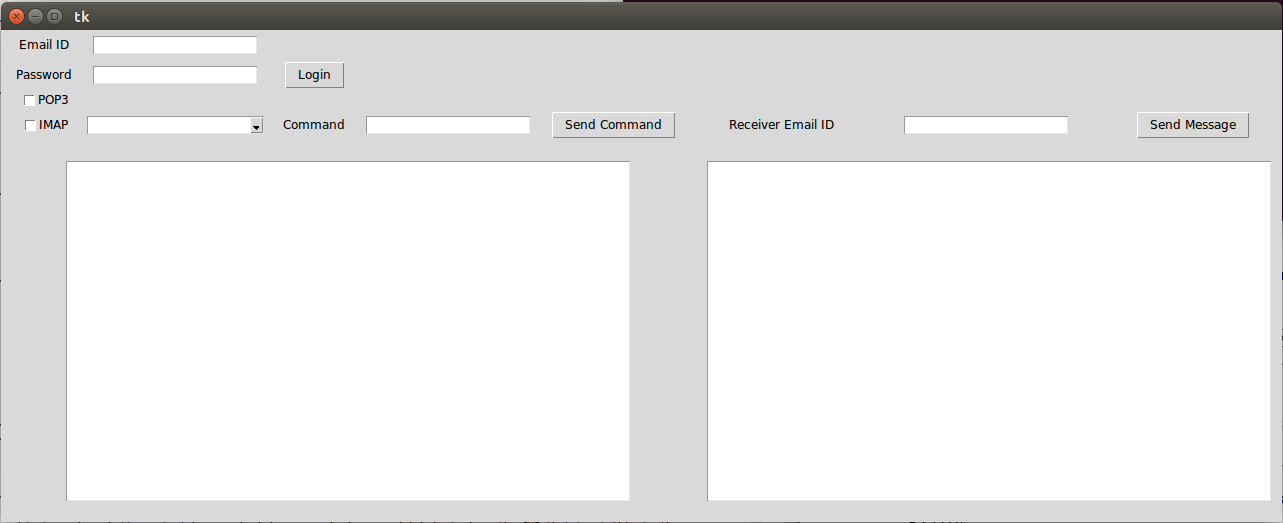
\includegraphics[scale=0.7]{images/MainSCreen.png}
\end{figure}

\begin{figure}[h]
\centering
\caption{Sending Message Screen}
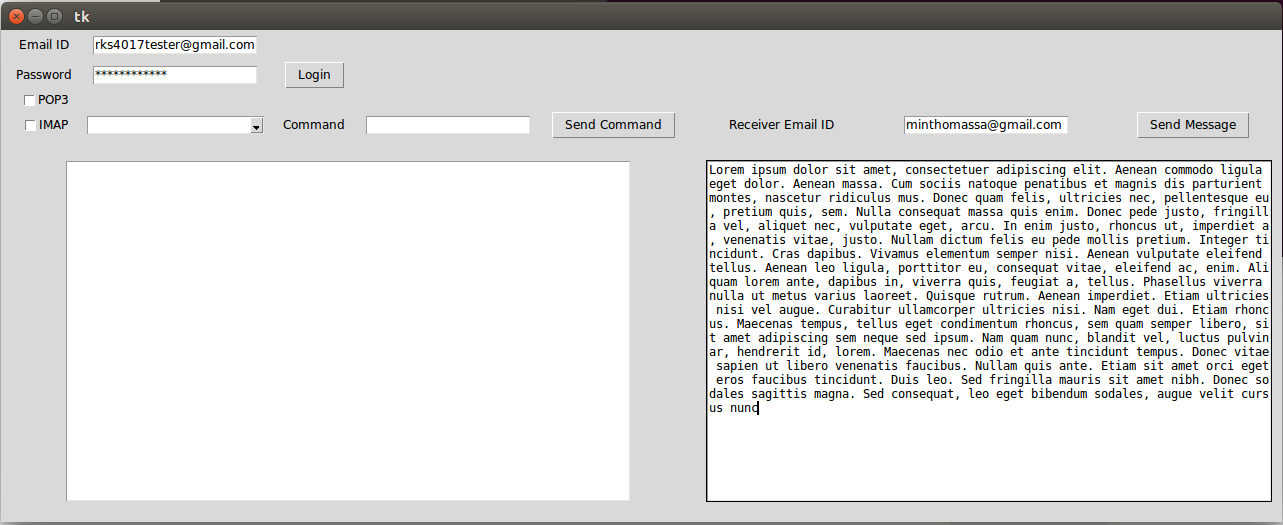
\includegraphics[scale=0.7]{images/sendingMessage.png}
\end{figure}

\begin{figure}[h]
\centering
\caption{Message Sent Screen}
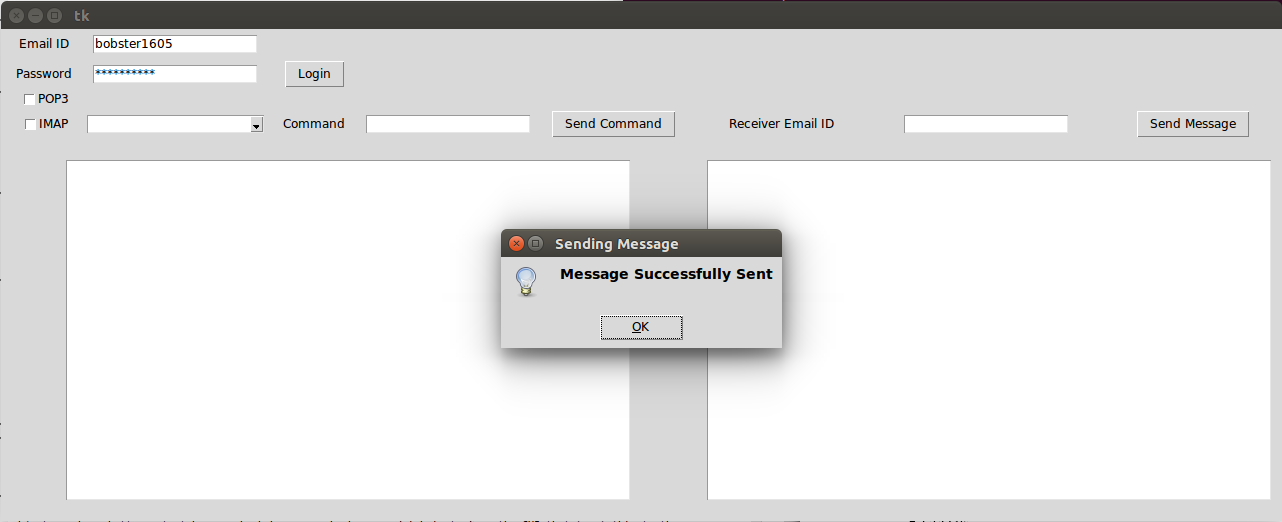
\includegraphics[scale=0.7]{images/messageSent.png}
\end{figure}

\begin{figure}[h]
\centering
\caption{IMAP Logged In Screen}
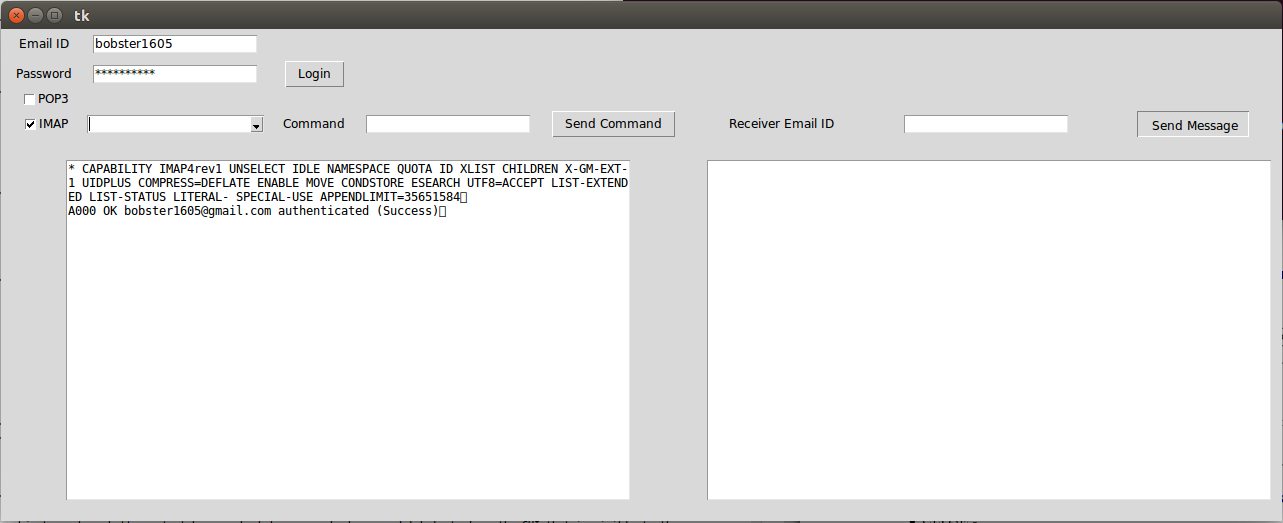
\includegraphics[scale=0.7]{images/IMAPloggedIn.png}
\end{figure}

\begin{figure}[!htb]
\centering
\caption{POP3 Logged In Screen}
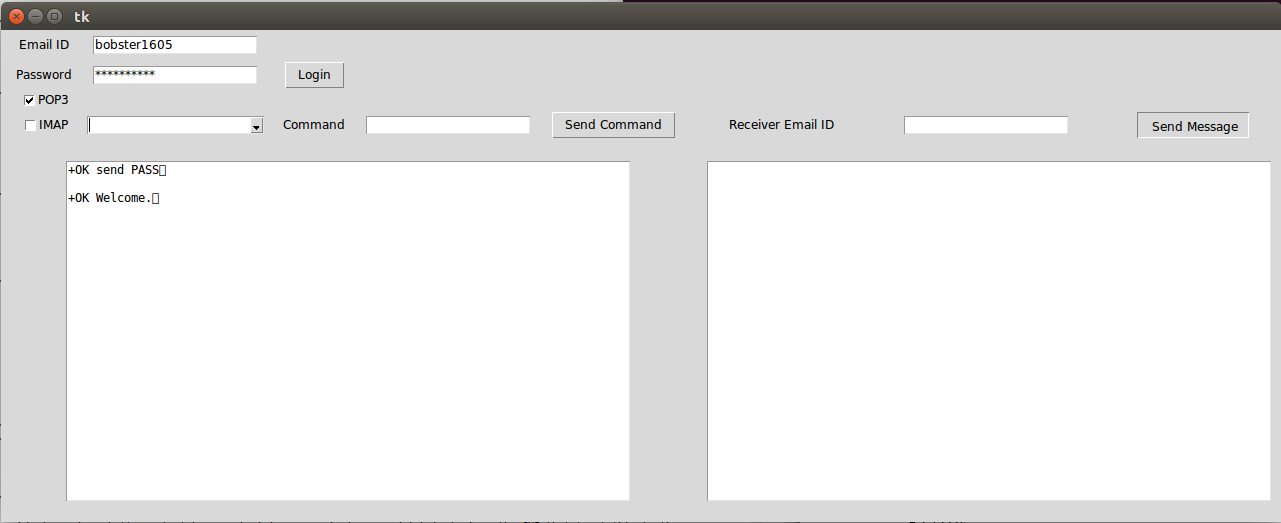
\includegraphics[scale=0.7]{images/POP3loggedIN.png}
\end{figure}

\begin{figure}[!htb]
\centering
\caption{POP3 Retrieve Message Screen}
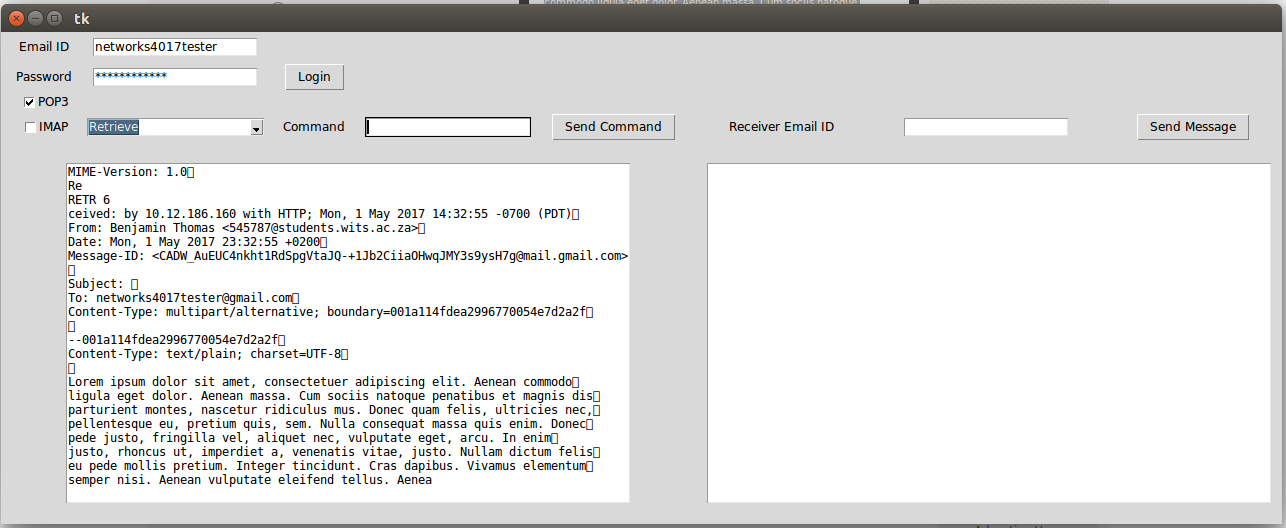
\includegraphics[scale=0.45]{images/receivedEmail.png}
\end{figure}

\newpage
\clearpage
\section{Appendix B: Wireshark Captures}
\begin{figure}[!htb]
\centering
\caption{Wireshark capture of SMTP client demonstration}
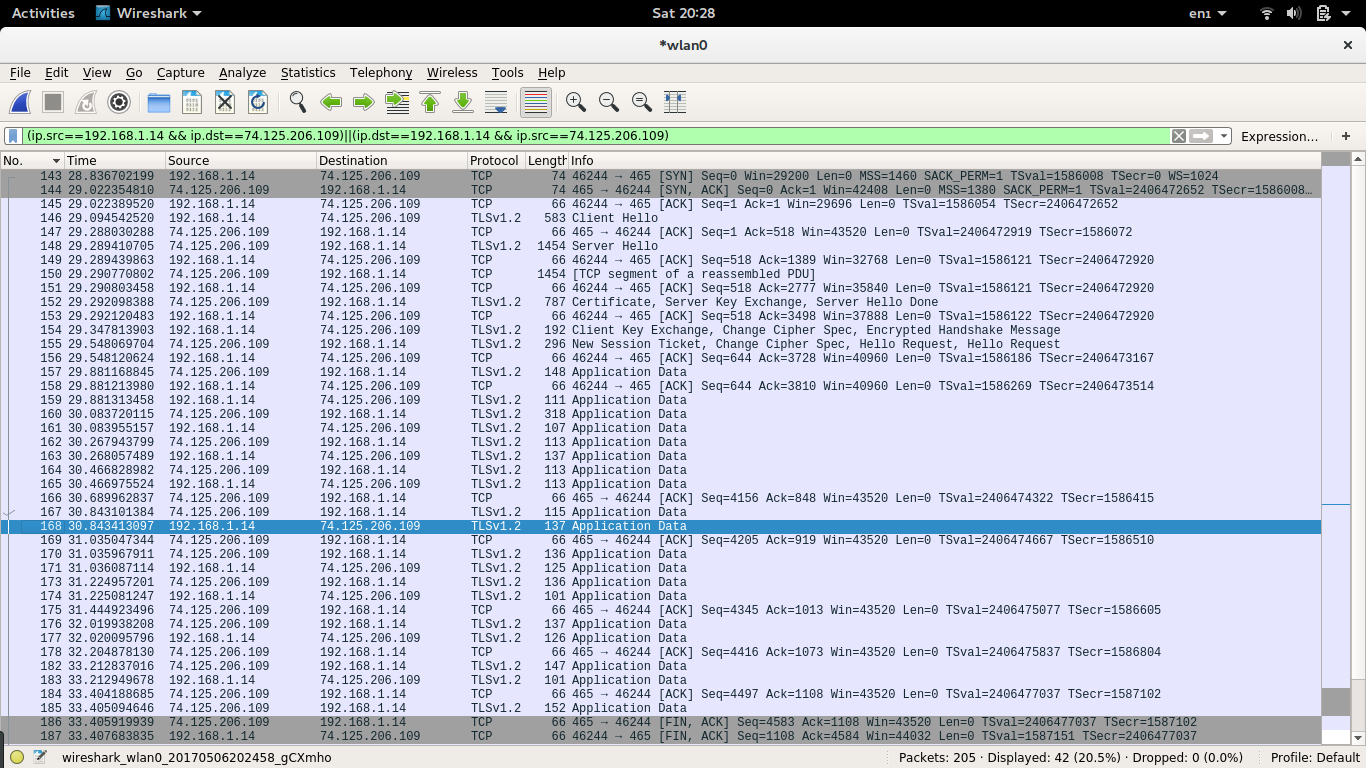
\includegraphics[width=17cm]{images/SMTP_CLIENT.png}
\label{SMTP_CLIENT}
\end{figure}

\begin{figure}[!htb]
\centering
\caption{Wireshark capture of SMTP server Demonstration}
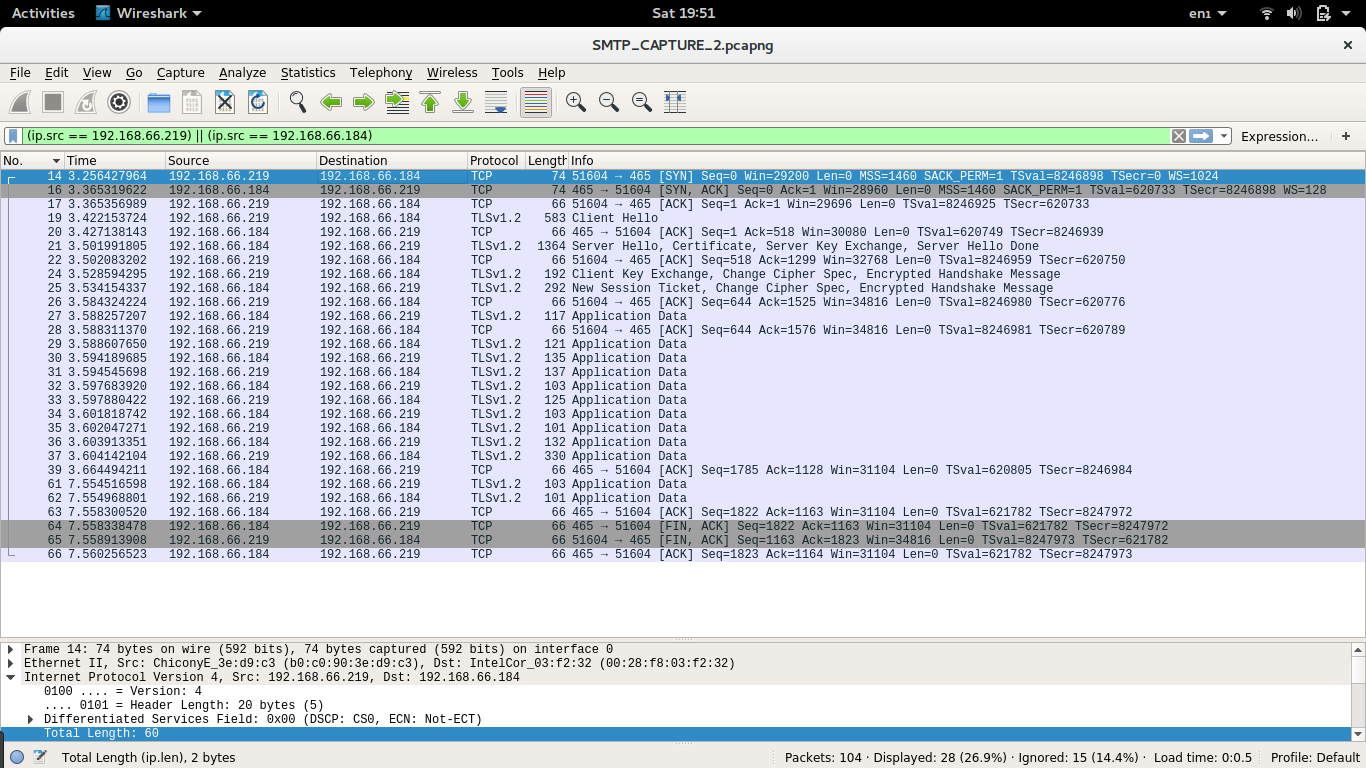
\includegraphics[width=17cm]{images/SMTP_SERVER.png}
\label{SMTP_SERVER}
\end{figure}

\begin{figure}[!htb]
\centering
\caption{Wireshark capture of IMAP client Demonstration}
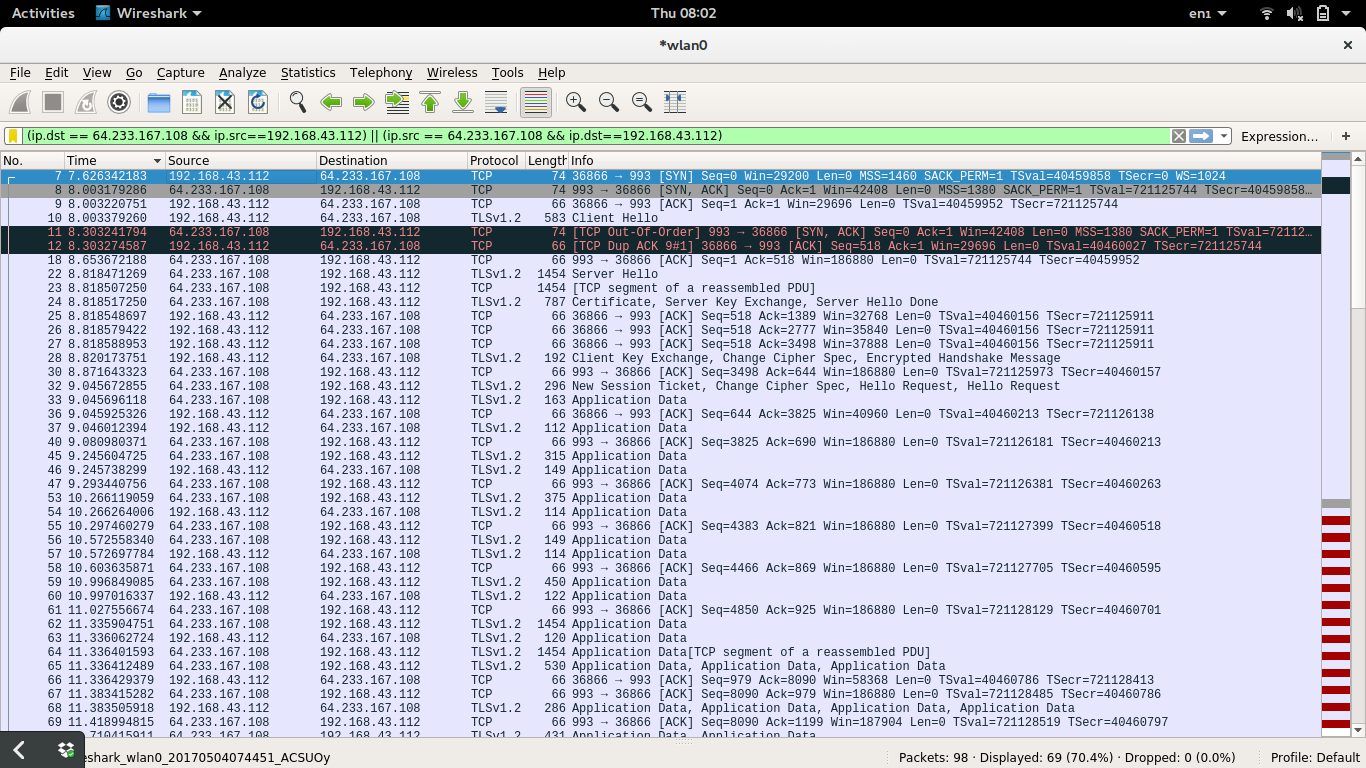
\includegraphics[width=17cm]{images/IMAP_CLIENT.png}
\label{IMAP_CLIENT}
\end{figure}

\begin{figure}[!htb]
\centering
\caption{Wireshark capture of IMAP server Demonstration}
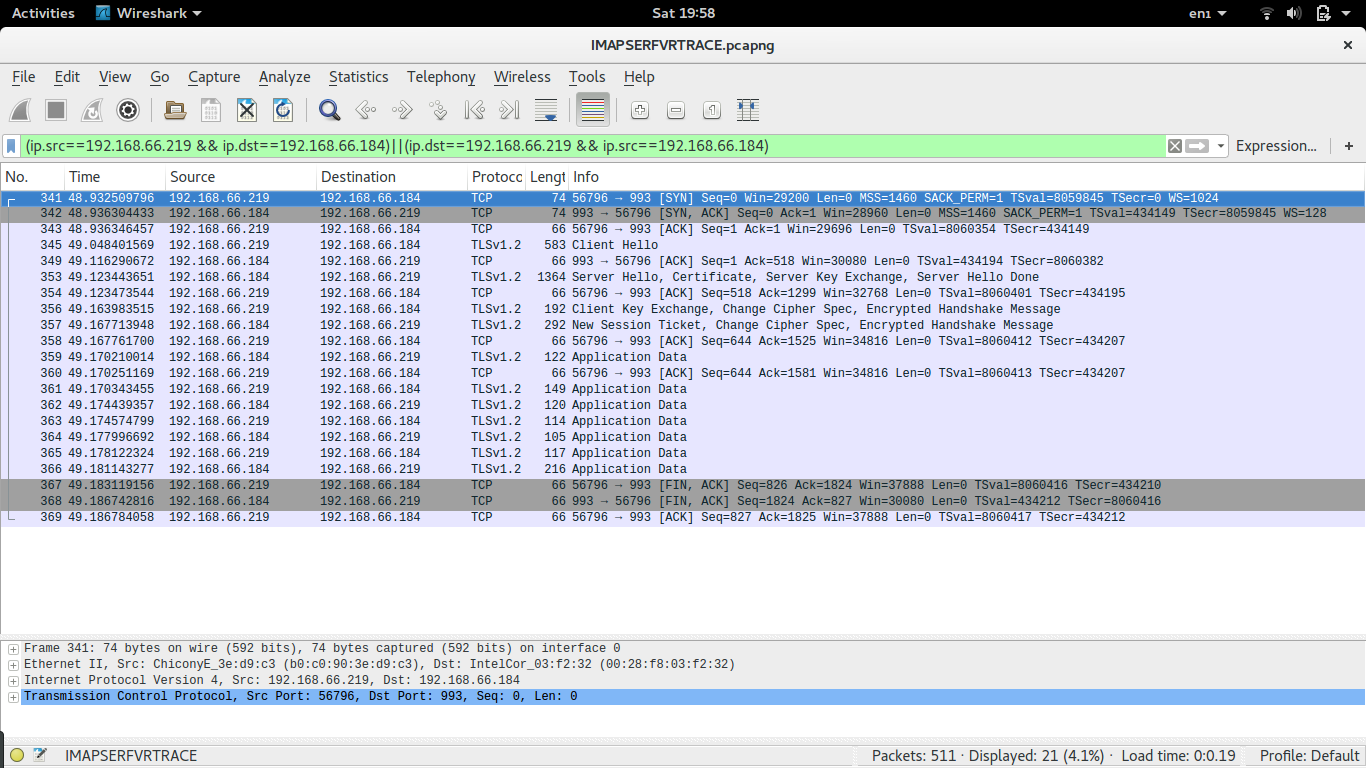
\includegraphics[width=17cm]{images/IMAP_SERVER.png}
\label{IMAP_SERVER}
\end{figure}


\end{document}


